
\documentclass[a4paper, 12pt]{article}
\usepackage[utf8]{inputenc}
\usepackage[T1]{fontenc}
\usepackage[slovak]{babel}
\usepackage{geometry}
\usepackage{graphicx}
\usepackage{svg}
\usepackage{url}
\usepackage{listings}
\usepackage{xcolor}
\usepackage{amsmath}
\usepackage{amssymb}
\usepackage[hidelinks,breaklinks=true]{hyperref}
\usepackage{booktabs}

\def\UrlBreaks{\do\/\do-\do.\do=\do?\do\&}
\Urlmuskip=0mu plus 1mu
\usepackage{multirow}
\usepackage{float}
\usepackage{subcaption}

\geometry{a4paper, left=2.5cm, right=2.5cm, top=2.5cm, bottom=2.5cm}

\lstset{
    basicstyle=\ttfamily\small,
    breaklines=true,
    frame=single,
    numbers=left,
    numberstyle=\tiny,
    showstringspaces=false,
    commentstyle=\color{gray},
    keywordstyle=\color{blue},
    stringstyle=\color{red}
}

\title{Tímový projekt \\ Virtual Data Analyst \\ Inteligentný systém pre analýzu dát pomocou prirodzeného jazyka}
\author{Peter Muzslay, Janka Tarčákova, Jana Kampová, Jozef Guláš, Tamara Uhrinová}
\date{Akademický rok 2025/2026}

\begin{document}

\maketitle
\clearpage
\tableofcontents
\clearpage

\section{Úvod}

Projekt \textbf{Virtuálny dátový analytik} predstavuje moderný webový systém, ktorý umožňuje používateľom analyzovať dáta v~databázach pomocou prirodzeného jazyka. Využitím pokročilých techník spracovania prirodzeného jazyka (NLP) a~veľkých jazykových modelov (LLM) dokáže systém transformovať otázky v~bežnom jazyku na SQL dotazy, vykonať ich nad databázou a~následne vrátiť zrozumiteľné odpovede.

Hlavným cieľom projektu je demokratizácia prístupu k~dátovej analytike -- umožniť aj netechnickým používateľom efektívne získavať informácie z~databáz bez potreby znalosti SQL alebo iných programovacích jazykov.

\subsection{Motivácia}

V~súčasnej dobe je dátová analytika kľúčovým faktorom pri rozhodovaní v~mnohých oblastiach podnikania. Avšak tradičné nástroje pre prácu s~databázami vyžadujú:
\begin{itemize}
    \item Znalosť SQL jazyka
    \item Pochopenie štruktúry databázy
    \item Technické zručnosti pre interpretáciu výsledkov
\end{itemize}

Virtuálny dátový analytik tieto bariéry odstraňuje a~sprístupňuje dátovú analýzu širšiemu okruhu používateľov.

\subsection{Štruktúra projektu}

Projekt je rozdelený do nasledujúcich hlavných komponentov:

\begin{enumerate}
    \item \textbf{Frontend} -- Používateľské rozhranie (React + Vite)
    \item \textbf{Backend} -- Serverová aplikácia (FastAPI, Python)
    \item \textbf{GenAI Core} -- Jadro pre spracovanie prirodzeného jazyka (LLM)
    \item \textbf{Databázová vrstva} -- Pripojenie a~správa databáz
\end{enumerate}

\clearpage

\section{Riešený problém}

\subsection{Definícia problému}

Hlavný problém, ktorý projekt rieši, je \textbf{preklad prirodzeného jazyka na štruktúrované databázové dotazy} a~následná \textbf{interpretácia výsledkov} pre koncového používateľa.

Konkrétne výzvy zahŕňajú:
\begin{itemize}
    \item \textbf{Sémantické porozumenie} -- Pochopenie zámeru používateľa z~neformálnej otázky
    \item \textbf{Mapovanie na schému} -- Správne priradenie entít v~otázke k~tabuľkám a~stĺpcom databázy
    \item \textbf{Generovanie validného SQL} -- Syntakticky a~sémanticky správne dotazy
    \item \textbf{Bezpečnosť} -- Zabezpečenie len čítacích operácií (READ-ONLY)
    \item \textbf{Zrozumiteľná odpoveď} -- Sumarizácia výsledkov v~prirodzenom jazyku
\end{itemize}

\subsection{Príklad použitia}

\begin{table}[H]
\centering
\begin{tabular}{p{6cm}p{8cm}}
\toprule
\textbf{Vstup (používateľ)} & \textbf{Výstup (systém)} \\
\midrule
„Koľko objednávok bolo vytvorených v~novembri 2019?" & Vygenerovaný SQL dotaz, počet záznamov a~textová sumarizácia výsledkov \\
\midrule
„Aký je priemerný počet položiek na objednávku?" & Analytický výsledok s~vysvetlením \\
\midrule
„Ukáž mi top 10 produktov podľa predaja" & Zoradený zoznam s~popisom \\
\bottomrule
\end{tabular}
\caption{Príklady interakcie s~virtuálnym analytikom}
\end{table}

\clearpage

\section{Prístup a~metodológia}

\subsection{Výber technológií}

Pri návrhu systému sme zvolili nasledujúce technológie:

\begin{table}[H]
\centering
\begin{tabular}{llp{7cm}}
\toprule
\textbf{Komponent} & \textbf{Technológia} & \textbf{Zdôvodnenie} \\
\midrule
Frontend & React + Vite & Moderný, reaktívny framework s~rýchlym vývojovým prostredím \\
Backend & FastAPI (Python) & Asynchrónne API s~automatickou dokumentáciou \\
Databáza & PostgreSQL & Robustná open-source relačná databáza \\
LLM & GPT-4.1 / Gemini 2.5 & Najmodernejšie jazykové modely pre NLP úlohy \\
Cache & Redis & In-memory databáza pre rýchle ukladanie do vyrovnávacej pamäte \\
Kontajnerizácia & Docker & Konzistentné prostredie pre vývoj a~nasadenie \\
\bottomrule
\end{tabular}
\caption{Použité technológie a~ich zdôvodnenie}
\end{table}

\subsection{Architektúra GenAI Core}

Jadro systému pre spracovanie prirodzeného jazyka pozostáva z~troch hlavných komponentov:

\begin{enumerate}
    \item \textbf{Router (LLM)} -- Rozhoduje o~spôsobe spracovania dotazu
    \item \textbf{Query Generator} -- Generuje SQL dotazy z~prirodzeného jazyka
    \item \textbf{Response Summarizer} -- Sumarizuje výsledky pre používateľa
\end{enumerate}

\subsubsection{Query Generator}

Komponent využíva model \texttt{GPT-4.1} pre generovanie SQL dotazov. Systémový prompt definuje pravidlá:
\begin{itemize}
    \item Generovať \textbf{len SELECT} dotazy (read-only prístup)
    \item Nikdy nepoužívať INSERT, UPDATE, DELETE, DROP, CREATE a~iné modifikačné príkazy
    \item Vrátiť len čistý SQL dotaz bez vysvetlení
    \item Používať správnu PostgreSQL syntax
\end{itemize}

\subsubsection{Response Summarizer}

Komponent využíva model \texttt{Gemini 2.5 Flash} pre sumarizáciu výsledkov. Poskytuje:
\begin{itemize}
    \item Popis, čo dáta zobrazujú
    \item Zvýraznenie kľúčových poznatkov a~vzorcov
    \item Zmienku o~významných hodnotách alebo trendoch
    \item Zrozumiteľný text pre netechnických používateľov
\end{itemize}

\clearpage

\section{Architektúra systému}

\subsection{Vysokoúrovňová architektúra (High-Level)}

Systém je navrhnutý ako \textbf{trojvrstvová architektúra} s~jasne oddelenými zodpovednosťami:

\begin{figure}[H]
\centering
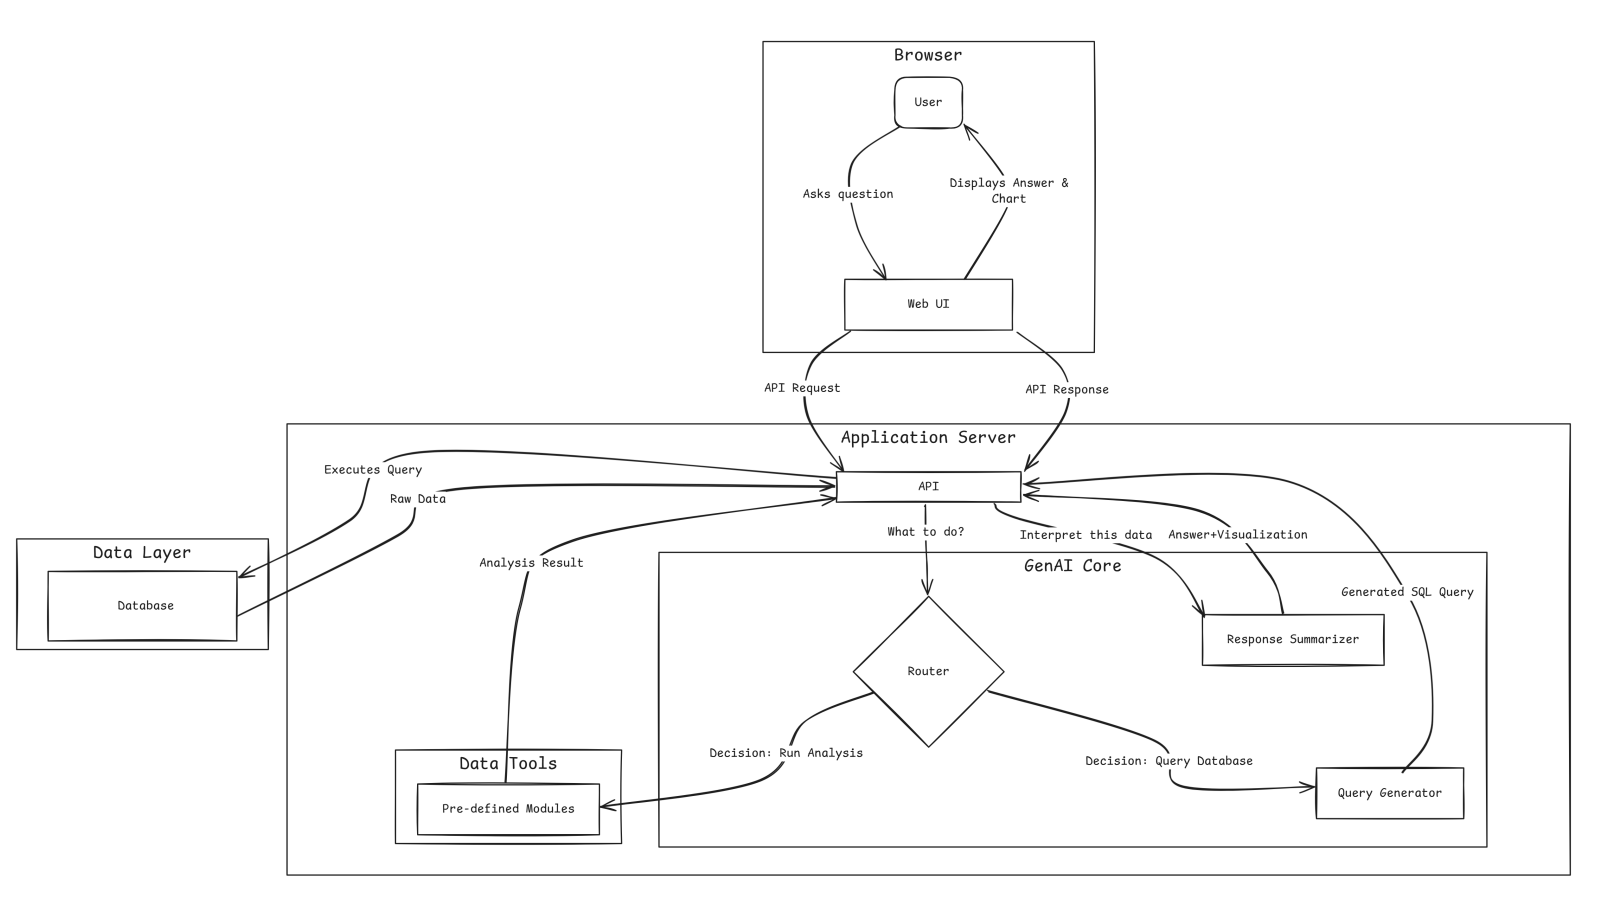
\includegraphics[width=1.05\textwidth]{high_level_VDA.png}
\caption{Vysokoúrovňová architektúra systému}
\end{figure}

\subsubsection{Tok dát (Data Flow)}

\begin{enumerate}
    \item Používateľ zadá otázku v~prirodzenom jazyku cez webové rozhranie
    \item Frontend odošle požiadavku na Backend API (\texttt{/api/ask})
    \item Backend získa schému databázy
    \item Query Generator (GPT-4.1) vygeneruje SQL dotaz
    \item Dotaz sa vykoná nad databázou (READ-ONLY)
    \item Response Summarizer (Gemini 2.5) vytvorí textovú sumarizáciu
    \item Odpoveď sa vráti používateľovi
\end{enumerate}

\clearpage

\subsection{Technická architektúra (Low-Level)}

\begin{figure}[H]
\centering
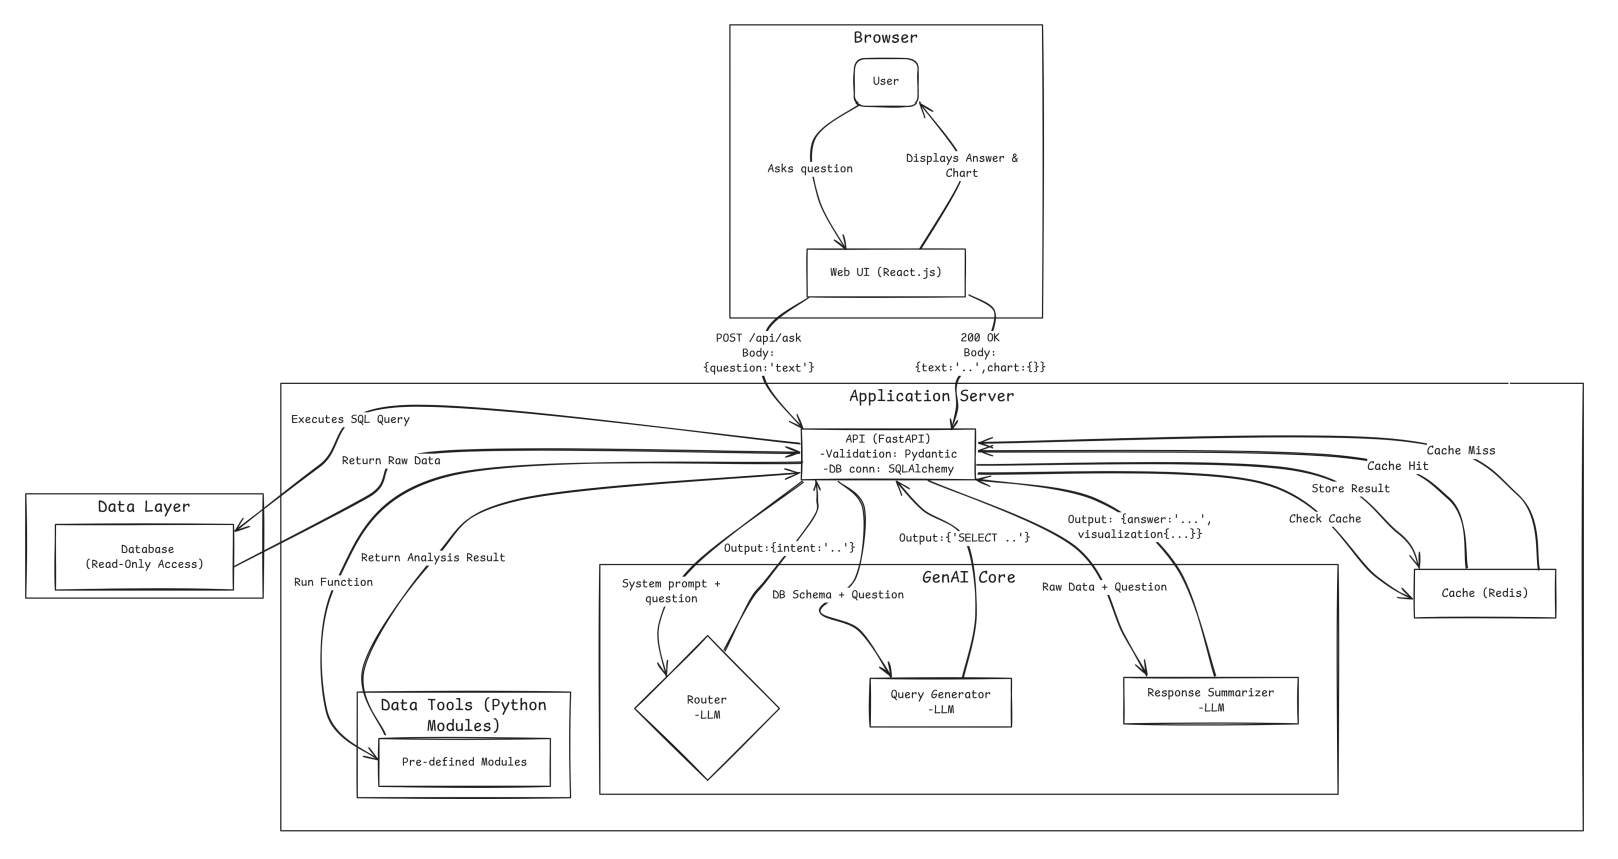
\includegraphics[width=1.05\textwidth]{arch_VDA.png}
\caption{Detailná architektúra systému s~komponentmi}
\end{figure}



\subsubsection{Backend komponenty}

\begin{table}[H]
\centering
\small
\begin{tabular}{lp{9cm}}
\toprule
\textbf{Komponent} & \textbf{Popis} \\
\midrule
\texttt{DatabaseManager} & Správa pripojenia k~PostgreSQL, vynucovanie READ-ONLY módu, získavanie schémy \\
\texttt{QueryGenerator} & LLM-based generovanie SQL dotazov pomocou GPT-4.1 \\
\texttt{ResponseSummarizer} & LLM-based sumarizácia výsledkov pomocou Gemini 2.5 Flash \\
\texttt{Router} & (TODO) Rozhodovanie medzi Data Tools a~Database queries \\
\texttt{RedisClient} & (TODO) Caching pre optimalizáciu opakovaných dotazov \\
\bottomrule
\end{tabular}
\caption{Backend komponenty a~ich zodpovednosti}
\end{table}

\subsubsection{API Endpoints}

\begin{table}[H]
\centering
\begin{tabular}{llp{6cm}}
\toprule
\textbf{Endpoint} & \textbf{Metóda} & \textbf{Popis} \\
\midrule
\texttt{/api/ask} & POST & Hlavný endpoint -- otázka $\rightarrow$ SQL $\rightarrow$ sumarizácia \\
\texttt{/api/generate-sql} & POST & Generovanie SQL bez vykonania \\
\texttt{/api/query-and-summarize} & POST & Vykonanie SQL a~sumarizácia \\
\texttt{/api/connect-database} & POST & Pripojenie k~databáze \\
\texttt{/api/disconnect-database} & POST & Odpojenie databázy \\
\texttt{/api/schema} & GET & Získanie schémy databázy \\
\bottomrule
\end{tabular}
\caption{REST API endpoints}
\end{table}

\subsubsection{Bezpečnostné mechanizmy}

Systém implementuje viacúrovňové zabezpečenie pre READ-ONLY prístup:

\begin{enumerate}
    \item \textbf{LLM Prompt} -- Systémový prompt zakazuje generovanie modifikačných príkazov
    \item \textbf{Regex validácia} -- Kontrola nebezpečných kľúčových slov (INSERT, UPDATE, DELETE, DROP...)
    \item \textbf{SQL Session} -- Nastavenie \texttt{SET TRANSACTION READ ONLY} na úrovni databázy
\end{enumerate}


\subsubsection{Frontend komponenty}

\begin{table}[H]
\centering
\begin{tabular}{lp{9cm}}
\toprule
\textbf{Komponent} & \textbf{Popis} \\
\midrule
\texttt{HomePage} & Hlavná stránka aplikácie, správa stavu pripojenia \\
\texttt{Chat} & Chat rozhranie pre komunikáciu s~analytikom \\
\texttt{SideBar} & Bočný panel s~ovládacími prvkami \\
\texttt{DatabaseModal} & Modal pre zadanie pripojovacích údajov k~databáze \\
\texttt{InputQuestion} & Vstupné pole pre zadávanie otázok \\
\texttt{UserMessage} & Zobrazenie správ v~chate \\
\bottomrule
\end{tabular}
\caption{React komponenty frontendu}
\end{table}

\clearpage

\section{Výber a~testovanie LLM modelov}

Pri návrhu systému bolo kľúčové rozhodnúť, ktoré veľké jazykové modely (LLM) použiť pre jednotlivé úlohy. Keďže systém vyžaduje dva odlišné typy spracovania -- generovanie SQL dotazov a~sumarizáciu výsledkov -- rozhodli sme sa pre špecializovaný prístup s~využitím rôznych modelov.

\subsection{Metodológia testovania}

Pre objektívne porovnanie výkonnosti LLM modelov sme vytvorili testovací skript, ktorý automatizovane vyhodnocoval schopnosti modelov riešiť SQL problémy. Ako zdroj testovacích úloh sme použili problémy z~platformy \textbf{HackerRank}, ktorá poskytuje široké spektrum SQL výziev rôznej obtiažnosti.

Testovací proces zahŕňal:
\begin{enumerate}
    \item \textbf{Kolekcia problémov} -- Výber 50+ SQL problémov z~HackerRank (easy, medium, hard)
    \item \textbf{Automatizované testovanie} -- Skript generoval dotazy pomocou každého modelu
    \item \textbf{Validácia výsledkov} -- Porovnanie vygenerovaných dotazov s~očakávanými výstupmi
    \item \textbf{Meranie metrík} -- Presnosť, čas odozvy, konzistencia výstupov
\end{enumerate}

\subsection{Porovnávané modely}

\begin{table}[H]
\centering
\begin{tabular}{ll}
\toprule
\textbf{Model} & \textbf{Poskytovateľ}  \\
\midrule
GPT-4.1 & OpenAI/Azure  \\
GPT-4o & OpenAI/Azure  \\
GPT-3.5-turbo & OpenAI/Azure  \\
Gemini 2.5 Flash & Google  \\
Gemini 2.5 Pro & Google  \\
Claude 4 Sonnet & Anthropic  \\
\bottomrule
\end{tabular}
\caption{Porovnávané LLM modely a~ich testované úlohy}
\end{table}

\subsection{Výsledky testovania -- SQL generácia}

Pre generovanie SQL dotazov sme testovali modely na nasledujúcich kritériách:

\begin{itemize}
    \item \textbf{Syntaktická správnosť} -- Percentuálna úspešnosť generovania validného SQL
    \item \textbf{Sémantická presnosť} -- Či dotaz vracia očakávané výsledky
    \item \textbf{Dodržiavanie pravidiel} -- Generovanie len READ-ONLY dotazov
    \item \textbf{Konzistencia} -- Stabilita výstupov pri opakovaných dotazoch
\end{itemize}

\textbf{GPT-4.1} dosiahol dobré výsledky v~syntaktickej aj sémantickej presnosti, pričom dosiahol aj dodržiavanie READ-ONLY pravidiel. Napriek vyššej latencii a mierne vyššej cene sme ho zvolili pre kritickú úlohu generovania SQL.

\subsection{Výsledky testovania -- Sumarizácia}

Pre sumarizáciu výsledkov sme hodnotili:

\begin{itemize}
    \item \textbf{Zrozumiteľnosť} -- Kvalita textu pre netechnických používateľov
    \item \textbf{Faktická správnosť} -- Presnosť interpretácie dát
    \item \textbf{Rýchlosť} -- Čas potrebný na generovanie odpovede
    \item \textbf{Cena} -- Náklady na API volania
\end{itemize}

\textbf{Gemini 2.5 Flash} ponúkol optimálny pomer kvality, rýchlosti a~ceny. Pri minimálnom rozdiele v~kvalite oproti drahším modelom poskytuje výrazne nižšiu latenciu, náklady a veľké kontextové okno.

\subsection{Záver výberu modelov}

Na základe testovania sme sa rozhodli pre kombináciu:

\begin{itemize}
    \item \textbf{GPT-4.1 (Azure)} pre generovanie SQL: dobrá presnosť a~spoľahlivosť pri dodržiavaní bezpečnostných pravidiel
    \item \textbf{Gemini 2.5 Flash (Vertex AI)} pre sumarizáciu: optimálny pomer veľkosť/cena/rýchlosť
\end{itemize}


\clearpage

\section{Použité technológie -- detailný prehľad}

\subsection{Backend technológie}

\subsubsection*{Python 3.12+}

Hlavný programovací jazyk aplikácie. Python je interpretovaný, vysokoúrovňový jazyk so silným ekosystémom knižníc pre dátovú vedu, strojové učenie a~webový vývoj. Verzia 3.12 prináša výrazné zlepšenia výkonu interprétera a~rozšírenú podporu asynchrónneho programovania. Vďaka jednoduchej syntaxi a~rozsiahlej komunite je Python de facto štandardom pre aplikácie využívajúce LLM modely a~AI integrácie. Jeho dynamická typovosť je dopĺňaná nástrojmi pre statickú analýzu, čo umožňuje kombináciu rýchlosti vývoja so spoľahlivosťou kódu.

\subsubsection*{FastAPI}

Moderný, asynchrónny webový framework pre budovanie REST API v~Pythone. FastAPI je postavený na štandarde ASGI a~knižnici Starlette, čo mu umožňuje natívne spracovávať asynchrónne požiadavky s~vysokou priepustnosťou. Automaticky generuje OpenAPI dokumentáciu na základe typových anotácií, čím výrazne znižuje objem manuálnej dokumentácie. Integrácia s~knižnicou Pydantic zabezpečuje automatickú validáciu vstupných a~výstupných dát. FastAPI patrí medzi najrýchlejšie Python frameworky pre webové API, čo ho robí vhodným pre aplikácie s~požiadavkami na nízku latenciu.

\subsubsection*{SQLAlchemy}

Komplexná knižnica pre prácu s~relačnými databázami v~Pythone, fungujúca ako ORM (Object-Relational Mapping) aj ako nástroj pre priame SQL operácie. Poskytuje jednotné rozhranie pre komunikáciu s~rôznymi databázovými systémami -- PostgreSQL, MySQL, MSSQL, Oracle a~ďalšími -- prostredníctvom systému dialektov. SQLAlchemy Inspector umožňuje introspekciu databázových metadát, čo aplikácia využíva na dynamické načítavanie schémy. Connection pooling zabudovaný v~SQLAlchemy efektívne spravuje životný cyklus databázových spojení a~znižuje réžiu pri opakovaných pripojeniach.

\subsubsection*{OpenAI SDK}

Oficiálna klientská knižnica pre komunikáciu s~OpenAI API a~kompatibilnými LLM endpointami. SDK poskytuje jednoduché rozhranie pre volanie modelov cez štandardizované Chat Completions API, pričom podporuje synchronné aj asynchrónne volania. Knižnica zabezpečuje správu HTTP spojení, serializáciu požiadaviek a~deserializáciu odpovedí vrátane štruktúrovaných výstupov. V~projekte sa používa nielen pre OpenAI modely (GPT-4.1), ale aj pre prístup k~modelom Google Gemini cez kompatibilný endpoint, čo umožňuje jednotné rozhranie pre viacero poskytovateľov LLM.

\subsubsection*{Pydantic}

Knižnica pre validáciu dát a~správu nastavení v~Pythone, postavená na typových anotáciách. Pydantic automaticky overuje typy, formáty a~obmedzenia vstupných dát pri ich spracovaní, čím predchádza chybám spôsobeným neplatnými vstupmi. V~kombinácii s~FastAPI definuje schémy pre API požiadavky a~odpovede, ktoré slúžia aj ako podklad pre automatickú OpenAPI dokumentáciu. Verzia 2 priniesla výrazné zlepšenie výkonu validácie a~rozšírenú podporu pre komplexné dátové modely. Pydantic Settings poskytuje typovo-bezpečné načítanie konfigurácie z~premenných prostredia.

\subsubsection*{uv}

Moderný správca Python balíčkov a~virtuálnych prostredí implementovaný v~jazyku Rust. Na rozdiel od tradičného nástroja pip je uv výrazne rýchlejší pri inštalácii závislostí vďaka paralelizácii a~agresívnemu cachovaniu. Podporuje správu závislostí cez súbor \texttt{pyproject.toml} a~deterministické zamykanie verzií cez \texttt{uv.lock}, čo zaručuje reprodukovateľné prostredie vo vývoji aj v~CI/CD pipeline. uv tiež zjednodušuje správu Python verzií a~virtuálnych prostredí v~jednom nástroji.


\subsection{Frontend technológie}


\subsubsection*{React}

JavaScriptová knižnica pre budovanie používateľských rozhraní. React zavádza komponentový model vývoja, kde sa UI skladá z~nezávislých, znovupoužiteľných komponentov s~vlastným stavom a~logikou. Virtuálny DOM zabezpečuje efektívne aktualizácie rozhrania tým, že minimalizuje priame manipulácie s~reálnym DOM stromom. Systém hookov (\texttt{useState}, \texttt{useEffect} a~ďalšie) umožňuje správu stavu a~vedľajších efektov vo funkcionálnych komponentoch bez potreby tried. React je v~súčasnosti jednou z~najrozšírenejších knižníc pre tvorbu webových aplikácií s~rozsiahlym ekosystémom doplnkov.

\subsubsection*{Vite}

Moderný build nástroj a~vývojový server pre JavaScript aplikácie. Vite využíva natívne ES moduly prehliadača počas vývoja, čo eliminuje potrebu bundlovania a~dramaticky skracuje čas štartu vývojového servera. Pre produkčné buildy používa Rollup, ktorý generuje optimalizované a~minifikované výstupy. Hot Module Replacement (HMR) v~prostredí Vite funguje takmer okamžite aj pri veľkých projektoch, čo výrazne zrýchľuje iteračný vývoj. Vite je navrhnutý ako nástupca starších nástrojov ako webpack a~Create React App.

\subsubsection*{Tailwind CSS}

Utility-first CSS framework, ktorý namiesto preddefinovaných komponentov poskytuje nízkoúrovňové CSS triedy aplikovateľné priamo v~HTML. Tento prístup eliminuje potrebu písania vlastných CSS súborov pre väčšinu prípadov a~vedie k~konzistentnejšiemu vizuálnemu dizajnu. Tailwind obsahuje rozsiahly systém designových tokenov pre farby, medzery, typografiu a~ďalšie vlastnosti. Produkčný build automaticky odstraňuje nepoužívané CSS triedy (tree-shaking), čím minimalizuje veľkosť výsledného CSS súboru. Responzívny dizajn je riešený pomocou prefixov breakpointov priamo v~triede.

\subsubsection*{Axios}

HTTP klientská knižnica pre JavaScript podporujúca požiadavky z~prehliadača aj z~prostredia Node.js. Axios poskytuje jednotné Promise-based API pre vykonávanie HTTP požiadaviek s~automatickou serializáciou JSON dát. Podporuje interceptory pre globálne spracovanie požiadaviek a~odpovedí, čo uľahčuje implementáciu autentifikácie a~centralizovaného spracovania chýb. Na rozdiel od natívneho \texttt{fetch} API automaticky odmietne Promise pri HTTP chybových stavoch (4xx, 5xx) a~poskytuje detailnejšie chybové objekty. V~projekte je nakonfigurovaný centrálny Axios klient so základnou URL adresou backendu a~spoločnými hlavičkami.


\subsection{Infraštruktúra}


\subsubsection*{Docker}

Platforma pre kontajnerizáciu aplikácií, ktorá zabaľuje aplikáciu a~všetky jej závislosti do izolovaného, prenosného kontajnera. Kontajnery zdieľajú jadro operačného systému hostiteľa, čo ich robí oveľa ľahšími ako tradičné virtuálne stroje. Dockerfile definuje sériu inštrukción pre zostavenie obrazu, čím zabezpečuje plne reprodukovateľné prostredie nezávislé od konfigurácie hostiteľského systému. Docker eliminuje problém „funguje to iba u~mňa" a~zjednodušuje nasadenie aplikácií na rôzne infraštruktúry. Je základným stavebným kameňom moderných CI/CD pipeline a~cloudových nasadení.

\subsubsection*{Docker Compose}

Nástroj pre definovanie a~spúšťanie viacerých Docker kontajnerov ako jednej aplikácie pomocou YAML konfiguračného súboru. Docker Compose umožňuje deklaratívne definovať služby, siete a~volumes, čo zjednodušuje orchestráciu komplexných aplikácií skladajúcich sa z~viacerých komponentov (backend, frontend, databáza, cache). Príkazom \texttt{docker compose up} sa spustia všetky služby s~ich závislosťami v~správnom poradí. V~projekte sa Docker Compose využíva nielen pre hlavnú aplikáciu, ale aj pre správu rôznych testovacích databáz, pričom každý databázový systém má vlastný konfiguračný súbor.

\subsubsection*{Redis}

In-memory databáza a~cache systém s~otvorených zdrojovým kódom, optimalizovaná pre extrémne rýchly prístup k~dátam. Redis ukladá dáta primárne v~operačnej pamäti, čo umožňuje časy odozvy v~rádoch mikrosekúnd. Podporuje rôzne dátové štruktúry -- reťazce, zoznamy, množiny, zoradené množiny a~hashe -- čo ho robí vhodným pre široké spektrum prípadov použitia od cachovania po správu frontov. TTL (Time-To-Live) mechanizmus umožňuje automatické vypršanie uložených dát, čo je kľúčové pre udržiavanie aktuálnosti cache. V~projekte Redis slúži pre štyri úrovne cachovania a~pre ukladanie sémantických embeddingov.

\subsection{AI/ML modely}

\begin{itemize}
    \item \textbf{GPT-4.1 (Azure)} -- Generovanie SQL dotazov
    \item \textbf{Gemini 2.5 Flash (Vertex AI)} -- Sumarizácia výsledkov
\end{itemize}

\clearpage

\section{Databázová vrstva}

Databázová vrstva predstavuje jednu zo základných súčastí aplikácie. Zabezpečuje pripojenie k~používateľovým SQL databázam, vynucovanie read-only prístupu, získavanie schémy a~vykonávanie dotazov. Okrem toho systém využíva dve ďalšie databázové technológie -- MongoDB pre perzistentnú históriu chatových relácií a~Redis pre viacúrovňové cachovanie.

\subsection{Podporované databázové systémy}

Aplikácia podporuje pripojenie k~nasledujúcim relačným databázovým systémom:

\begin{itemize}
    \item \textbf{PostgreSQL} -- primárne testovaná a~podporovaná databáza,
    \item \textbf{MySQL} -- podpora cez pymysql konektor,
    \item \textbf{Microsoft SQL Server} -- podpora cez pyodbc a~odbc driver,
    \item \textbf{Oracle Database} -- podpora cez python-oracledb.
\end{itemize}

Typ databázy používateľ zadáva pri pripájaní. Backend na základe neho zostaví správny connection string a~zvolí príslušný SQLAlchemy dialekt. Aplikácia zároveň automaticky konfiguruje bezpečnostné mechanizmy špecifické pre daný dialekt.

\subsection{Správa databázového pripojenia}

Správa pripojenia je centralizovaná v~samostatnej komponente \texttt{DatabaseManager}, ktorá zapuzdruje celý životný cyklus spojenia -- od inicializácie až po odpojenie. Komponenta je postavená na SQLAlchemy ORM a~všetky jej operácie sú implementované asynchrónne, čo umožňuje paralelné spracovanie viacerých požiadaviek bez blokovania aplikácie.

Pre efektívne využívanie zdrojov je použitý \textbf{connection pool} -- sada trvalých pripojení udržiavaných na pozadí. Pool zabezpečuje automatické obnovenie zlyhajúcich spojení a~obmedzuje počet súbežných pripojení k~databáze. Pred každým použitím spojenia sa overuje jeho platnosť, čím sa predchádza chybám pri výpadkoch siete.

\subsubsection{Získavanie schémy}

Po pripojení systém načíta štruktúru databázy priamo z~jej systémových metadát. Pre každú tabuľku získa zoznam stĺpcov vrátane ich názvov, dátových typov a~informácie o~tom, či stĺpec môže obsahovať prázdnu hodnotu. Takto získaná schéma slúži ako kontext pre LLM model -- model dostane úplný prehľad tabuliek a~stĺpcov, aby mohol generovať syntakticky a~sémanticky správne dotazy.

\subsubsection{Vykonávanie dotazov}

Dotazy sa vykonávajú výhradne v~read-only režime. Bezpečnosť je zaistená na troch úrovniach, ktoré sú popísané v~nasledujúcej podsekcii. Výsledky dotazu sú vrátené ako štruktúrovaný zoznam záznamov, kde každý záznam obsahuje hodnoty stĺpcov pod ich názvami.

\subsection{READ-ONLY prístup a~bezpečnosť}

Jeden z~najdôležitejších aspektov databázovej vrstvy je garantovaný read-only prístup. Ochrana je implementovaná na troch nezávislých úrovniach:

\begin{enumerate}
    \item \textbf{Úroveň jazykového modelu} -- systémový prompt pre SQL generátor výslovne zakazuje generovanie akýchkoľvek modifikačných príkazov a~povoľuje výlučne príkazy SELECT,
    \item \textbf{Úroveň regulárnych výrazov} -- pred vykonaním sa každý dotaz skontroluje na prítomnosť nebezpečných kľúčových slov (INSERT, UPDATE, DELETE, DROP, CREATE, ALTER, TRUNCATE, GRANT, REVOKE); detekcia je nezávislá od veľkosti písmen a~pri nájdení zakázaného slova sa dotaz odmietne,
    \item \textbf{Úroveň databázovej transakcie} -- pre podporované databázové systémy sa read-only mód nastaví priamo na úrovni databázovej transakcie pomocou databázo-špecifického príkazu.
\end{enumerate}

Tento trojúrovňový prístup zabezpečuje, že ani pri kompromitácii jednej vrstvy nedôjde k~nežiaducim zmenám v~databáze.

\subsection{Parametrizácia pripojenia}

Aplikácia umožňuje dynamické pripojenie na ľubovoľnú databázu bez zmeny kódu. Používateľ zadáva nasledujúce parametre:

\begin{table}[H]
\centering
\begin{tabular}{ll}
\toprule
\textbf{Parameter} & \textbf{Popis} \\
\midrule
Typ databázy & Dialekt (PostgreSQL, MySQL, SQL Server, Oracle) \\
Host & Hostname alebo IP adresa servera \\
Port & Port, na ktorom databázový server počúva \\
Používateľské meno & Prihlasovacie meno \\
Heslo & Prístupové heslo \\
Názov databázy & Meno databázy alebo service name (Oracle) \\
\bottomrule
\end{tabular}
\caption{Parametre pre pripojenie k~databáze}
\end{table}

Backend tieto parametre skombinuje do connection stringu kompatibilného s~príslušným dialektom, inicializuje databázové pripojenie a~zároveň vytvorí novú reláciu v~MongoDB pre históriu chatu. Pri odpojení sa uzavrie databázové spojenie aj MongoDB session.

\subsection{API endpointy pre správu pripojenia}

\begin{table}[H]
\centering
\begin{tabular}{llp{7cm}}
\toprule
\textbf{Endpoint} & \textbf{Metóda} & \textbf{Popis} \\
\midrule
\texttt{/api/connect-database} & POST & Pripojenie k~databáze, vytvorenie MongoDB session \\
\texttt{/api/disconnect-database} & POST & Odpojenie, uzavretie session, vyčistenie cache \\
\texttt{/api/schema} & GET & Vrátenie aktuálnej schémy databázy \\
\bottomrule
\end{tabular}
\caption{Endpointy pre správu databázového pripojenia}
\end{table}

\subsection{Testovacie databázy a~Docker Compose}

Pre vývoj a~testovanie aplikácie je pripravených niekoľko samostatných Docker Compose konfigurácií, každá so svojím datasetom:

\begin{table}[H]
\centering
\begin{tabular}{ll}
\toprule
\textbf{Konfigurácia} & \textbf{Obsah} \\
\midrule
PostgreSQL -- e-commerce & Zákaznícke správanie v~e-commerce prostredí \\
PostgreSQL -- bike store & Predajné dáta obchodu s~bicyklami \\
MySQL -- e-commerce & E-commerce analýza v~MySQL dialekte \\
Microsoft SQL Server & Testovacia databáza pre enterprise prostredie \\
Oracle Database & Testovacia databáza pre korporátne prostredie \\
\bottomrule
\end{tabular}
\caption{Testovacie databázy pre vývoj}
\end{table}

Každá konfigurácia obsahuje health check pre monitorovanie dostupnosti, automatickú inicializáciu dát zo SQL skriptov a~CSV súborov a~persistentné volumes pre ukladanie dát medzi reštartmi kontajnera.

\subsection{MongoDB -- história chatových relácií}

Pre perzistentnú históriu konverzácií systém využíva MongoDB. Každá databázová session má vlastný dokument obsahujúci metadáta o~pripojení (typ databázy, host, názov databázy, čas pripojenia a~odpojenia) a~pole správ konverzácie. Každá správa uchováva rolu (používateľ alebo asistent), textový obsah, prípadný SQL dotaz, počet vrátených riadkov a~časovú pečiatku.

\begin{lstlisting}[language=Python, caption={štruktúra MongoDB session}]
{
  "session_id": "uuid",
  "user_id": "...",
  "db_type": "postgresql",
  "db_host": "...",
  "db_name": "...",
  "connected_at": "datetime",
  "disconnected_at": None,
  "messages": [
    {
      "role": "user" | "assistant",
      "content": "...",
      "sql_query": "...",
      "row_count": 42,
      "success": True,
      "timestamp": "datetime"
    }
  ]
}
\end{lstlisting}

Pre rýchly prístup sú vytvorené indexy na identifikátor session a~na kombináciu identifikátora používateľa s~časom pripojenia, čo umožňuje efektívne načítanie zoznamu relácií zoradených od najnovšej.

História relácií sa využíva v~dvoch smeroch: frontend ju zobrazuje používateľovi v~sidebare, a~backend z~nej extrahuje kontext pre LLM model pri generovaní SQL dotazov.

\subsubsection{Kontext pre SQL generátor}

Pri každom dopyte systém načíta históriu aktuálnej relácie a~pripraví z~nej kontext pozostávajúci z troch zložiek: 

 \begin{itemize}
     \item textová reprezentácia posledných správ konverzácie
     \item posledný vygenerovaný SQL dotaz
     \item osledná otázka používateľa
 \end{itemize} 

Tento kontext je odovzdaný SQL generátoru, ktorý ho zahrnie do promptu. Vďaka tomu model rozumie nadväzujúcim otázkam -- napríklad ak používateľ najprv spýta „ukáž posledné objednávky" a~následne „teraz len top 10", model vie o~predchádzajúcom dotaze a~sformuluje správny SQL.

\subsection{Redis -- cachovanie}

Pre zrýchlenie opakovaných operácií systém využíva Redis ako in-memory cache. Implementované sú štyri úrovne cachovania:

\begin{table}[H]
\centering
\small
\begin{tabular}{lp{5.5cm}p{4cm}}
\toprule
\textbf{Cache} & \textbf{Obsah} & \textbf{Kľúč} \\
\midrule
Schéma & Štruktúra databázy (tabuľky a~stĺpce) & prefix + odtlačok databázy \\
NL2SQL & Vygenerovaný SQL pre danú otázku & prefix + odtlačok DB + hash signatúry otázky \\
Výsledky SQL & Výsledky vykonaného dotazu & prefix + odtlačok DB + hash SQL \\
Sumarizácia & Textová sumarizácia výsledkov & prefix + odtlačok DB + hash SQL + hash otázky \\
\bottomrule
\end{tabular}
\caption{Úrovne Redis cache}
\end{table}

Každá cache vrstva funguje na princípe \textbf{cache-aside}: najprv sa pokúsi načítať dáta z~Redisu, pri cache miss vykoná skutočnú operáciu (volanie databázy alebo LLM) a~výsledok uloží do Redisu s~nastaveným TTL. Cache kľúče obsahujú krátky hash connection stringu databázy, čo zabezpečuje, že cache z~jednej databázy sa nikdy nepoužije pre inú.

\subsubsection{Sémantická Q\&A cache}

Nad štandardným cachovaním je implementovaná sémantická cache pre celé dvojice otázka-odpoveď. Pri každom úspešnom spracovaní otázky sa uloží vektorová reprezentácia (embedding) otázky spolu s~SQL dotazom, sumarizáciou a~počtom riadkov.

Pri ďalšom dopyte systém porovná embedding novej otázky s~uloženými pomocou cosine similarity. Ak podobnosť prekročí nakonfigurovaný prah, vráti uloženú odpoveď okamžite -- bez volania LLM modelu ani databázy. Sémantická cache navyše overuje zhodu kľúčových slov a~číselných hodnôt v~otázke, aby zabránila falošným hitom pri otázkach s~rôznymi filtrami alebo hodnotami.

\subsubsection{Cache metriky a~diagnostika}

Systém sleduje počty cache hitov a~missov pre každú vrstvu v~Redise. Každá odpoveď z~API obsahuje HTTP hlavičky s~informáciami o~stave cache:

\begin{itemize}
    \item \texttt{X-Cache-Schema} -- HIT alebo MISS pre schému databázy,
    \item \texttt{X-Cache-NL2SQL} -- HIT alebo MISS pre SQL generovanie,
    \item \texttt{X-Cache-SQL-Results} -- HIT alebo MISS pre výsledky dotazu,
    \item \texttt{X-Cache-Summary} -- HIT alebo MISS pre sumarizáciu,
    \item \texttt{X-Cache-QA-Semantic} -- HIT alebo MISS pre sémantickú cache,
    \item \texttt{X-Cache-Trace} -- zhrnutie všetkých cache stavov v~jednej hlavičke.
\end{itemize}

Tieto hlavičky umožňujú rýchlu diagnostiku výkonu systému priamo z~HTTP klienta alebo vývojárskych nástrojov prehliadača.

\clearpage

\section{Frontendová časť aplikácie}

\subsubsection{Štruktúra projektu}

Frontendová časť aplikácie je implementovaná pomocou knižnice React v kombinácii s nástrojom Tailwind. Projekt je rozdelený do modulov, aby bol prehľadný a komponenty sa dali ľahko znovu použiť. Komponenty sú navrhnuté tak, aby boli čo najviac nezávislé a komunikovali medzi sebou prostredníctvom vlastností (props).

Adresárová štruktúra projektu je nasledovná:

\begin{itemize}
    \item \texttt{components/} - Komponenty, ktoré tvoria používateľské rozhranie, napríklad chat, bočný panel, modálne okná a vstupné polia.
    \item \texttt{hooks/} - Vlastné React hooky, ktoré riešia logiku aplikácie, napríklad pripojenie k databáze.
    \item \texttt{services/} - Funkcie na komunikáciu s backendom.
    \item \texttt{pages/} - Komponenty pre hlavné stránky aplikácie.
    \item \texttt{assets/} - Obrázky, ikony a iné statické súbory.
    \item \texttt{api/} - Nastavenie HTTP klienta pre volania na backend.
\end{itemize}

\subsubsection{Správa stavu aplikácie}

Správa stavu aplikácie je realizovaná pomocou vstavaných React hookov \texttt{useState}, \texttt{useEffect} a \texttt{useRef}.

Stavy sú spravované lokálne v jednotlivých komponentoch, napríklad:
\begin{itemize}
    \item otvorenie a zatvorenie modálneho okna pre databázu,
    \item stav načítavania počas pripájania databázy,
    \item vstupné hodnoty formulárových polí,
    \item priebeh komunikácie v chatovom rozhraní.
\end{itemize}

\subsubsection{Vlastné React hooky}

Vo fronte je použitý vlastný React hook \texttt{useDatabase}, ktorý sa stará o pripojenie a odpojenie databázy. Komponenty ho môžu použiť bez toho, aby sa museli starať o detaily HTTP komunikácie.  

Hook \texttt{useDatabase}:
\begin{itemize}
    \item pripája a odpojuje databázu cez backend,
    \item sleduje, či sa práve načítava (\texttt{loading}),
    \item uchováva a zobrazuje chyby (\texttt{error}),
\end{itemize}


\subsection{Komunikácia s backendom}

Frontendová aplikácia komunikuje s backendom prostredníctvom HTTP požiadaviek. 
Táto komunikácia zabezpečuje pripojenie a odpojenie databázy, ako aj odosielanie otázok používateľa a prijímanie odpovedí od systému. Frontend odosiela požiadavky na backend vo formáte JSON a backend vracia odpovede v rovnakom formáte.

\subsubsection{Správa API volaní pomocou Axios}

Pre komunikáciu s backendom je použitá knižnica \textbf{Axios}. 
V projekte je vytvorený jeden centrálny Axios klient, ktorý obsahuje základnú konfiguráciu, ako je adresa backendového servera a hlavičky požiadaviek.

\begin{lstlisting}[caption={Základná konfigurácia Axios klienta}]
import axios from "axios";

const api = axios.create({
  baseURL: import.meta.env.VITE_API_BASE_URL || "http://localhost:8000",
  headers: {
    "Content-Type": "application/json",
  },
});

export default api;
\end{lstlisting}

Na základe tohto klienta sú vytvorené servisné funkcie, ktoré reprezentujú jednotlivé API volania.

\begin{lstlisting}[caption={Servisné funkcie pre komunikáciu s backendom}]
import api from "./api";

export const connectDatabase = async (data) => {
  const response = await api.post("/api/connect-database", data);
  return response.data;
};

export const disconnectDatabase = async () => {
  const response = await api.post("/api/disconnect-database");
  return response.data;
};

export const askQuestion = async (question) => {
  const response = await api.post("/api/ask", {
    question,
  });
  return response.data;
};
\end{lstlisting}

\subsection{Používateľské rozhranie}

Frontendová aplikácia má jednoduché a prehľadné rozhranie, ktoré umožňuje používateľovi komunikovať so systémom a spravovať pripojenie k databáze.

\subsubsection{Rozloženie aplikácie}

Hlavná stránka je rozdelená na dve časti:

\begin{itemize}
    \item \textbf{Bočný panel (Sidebar)} - obsahuje tlačidlá na otvorenie modálu pre pripojenie k databáze a ďalšie ovládacie prvky.
    \item \textbf{Hlavný obsah (Chat)} - zobrazujú sa správy medzi používateľom a systémom.
\end{itemize}

\begin{figure}[H]
\centering
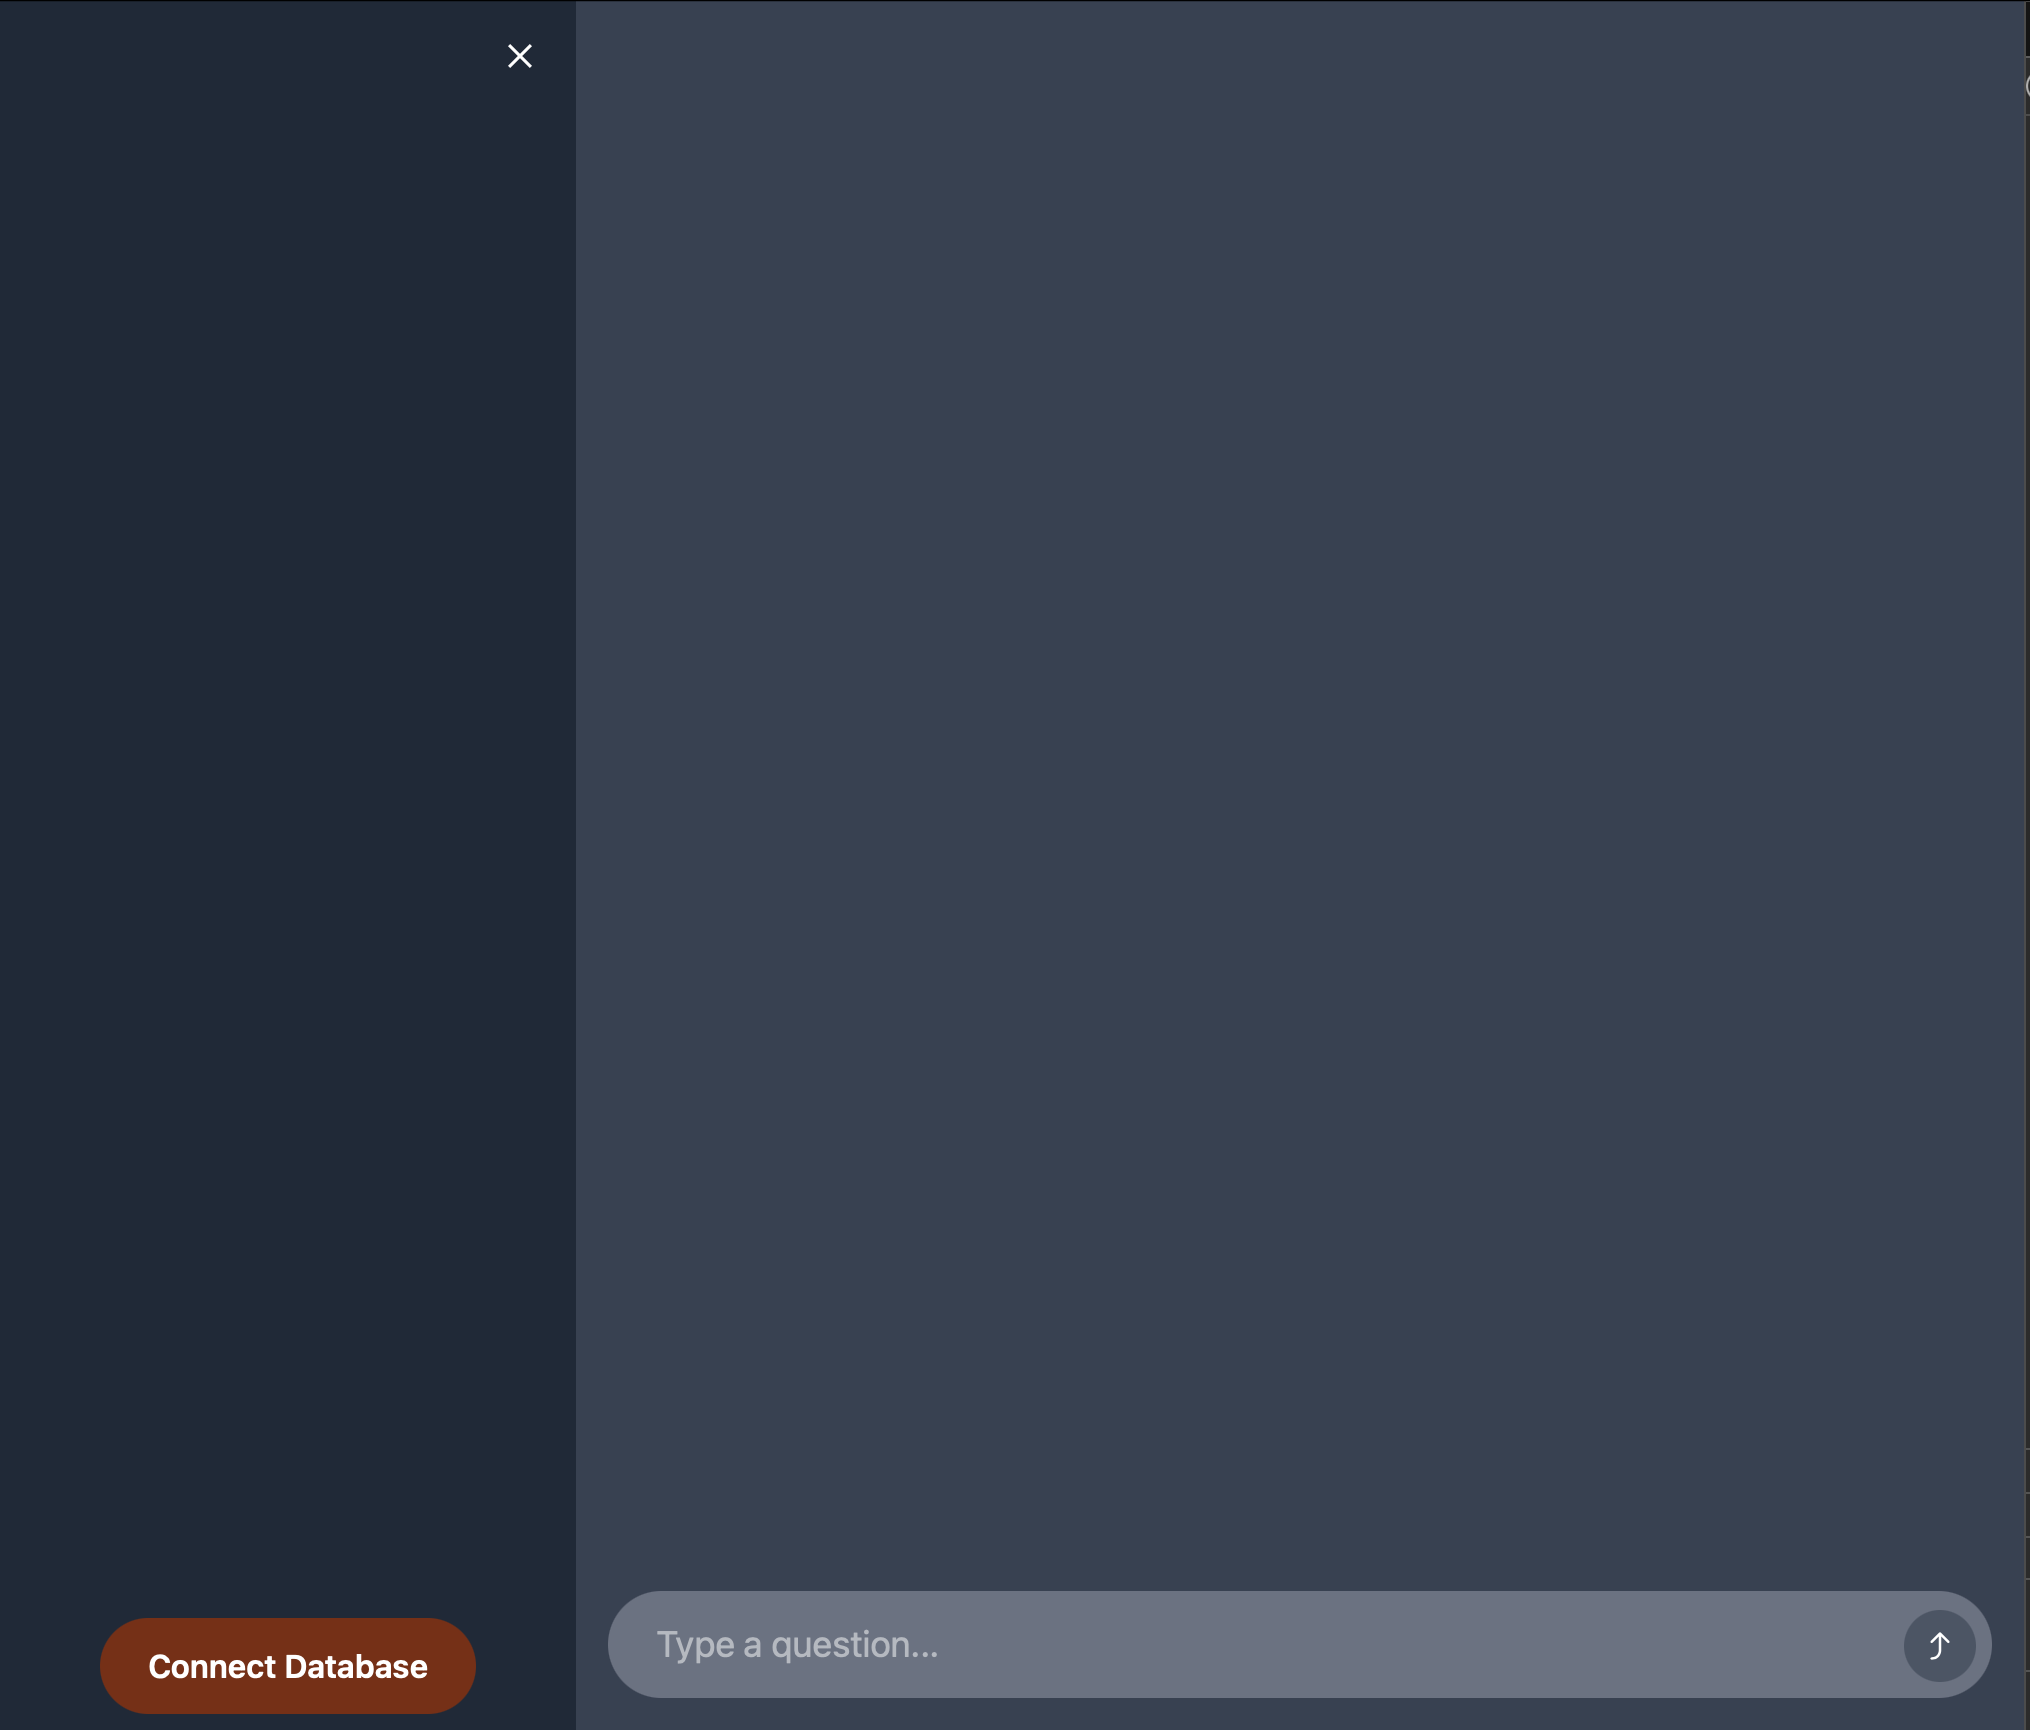
\includegraphics[width=0.95\textwidth]{frontend_layout.png}
\caption{Ukážka rozloženia frontendovej aplikácie}
\end{figure}
\clearpage
\subsubsection{Chatové rozhranie}

Chat pozostáva z oblasti správ a vstupného poľa na zadávanie otázok. Používateľ môže zadávať otázky, ktoré sú posielané systému, a výsledky sa zobrazujú v chronologickom poradí.


\begin{figure}[H]
\centering
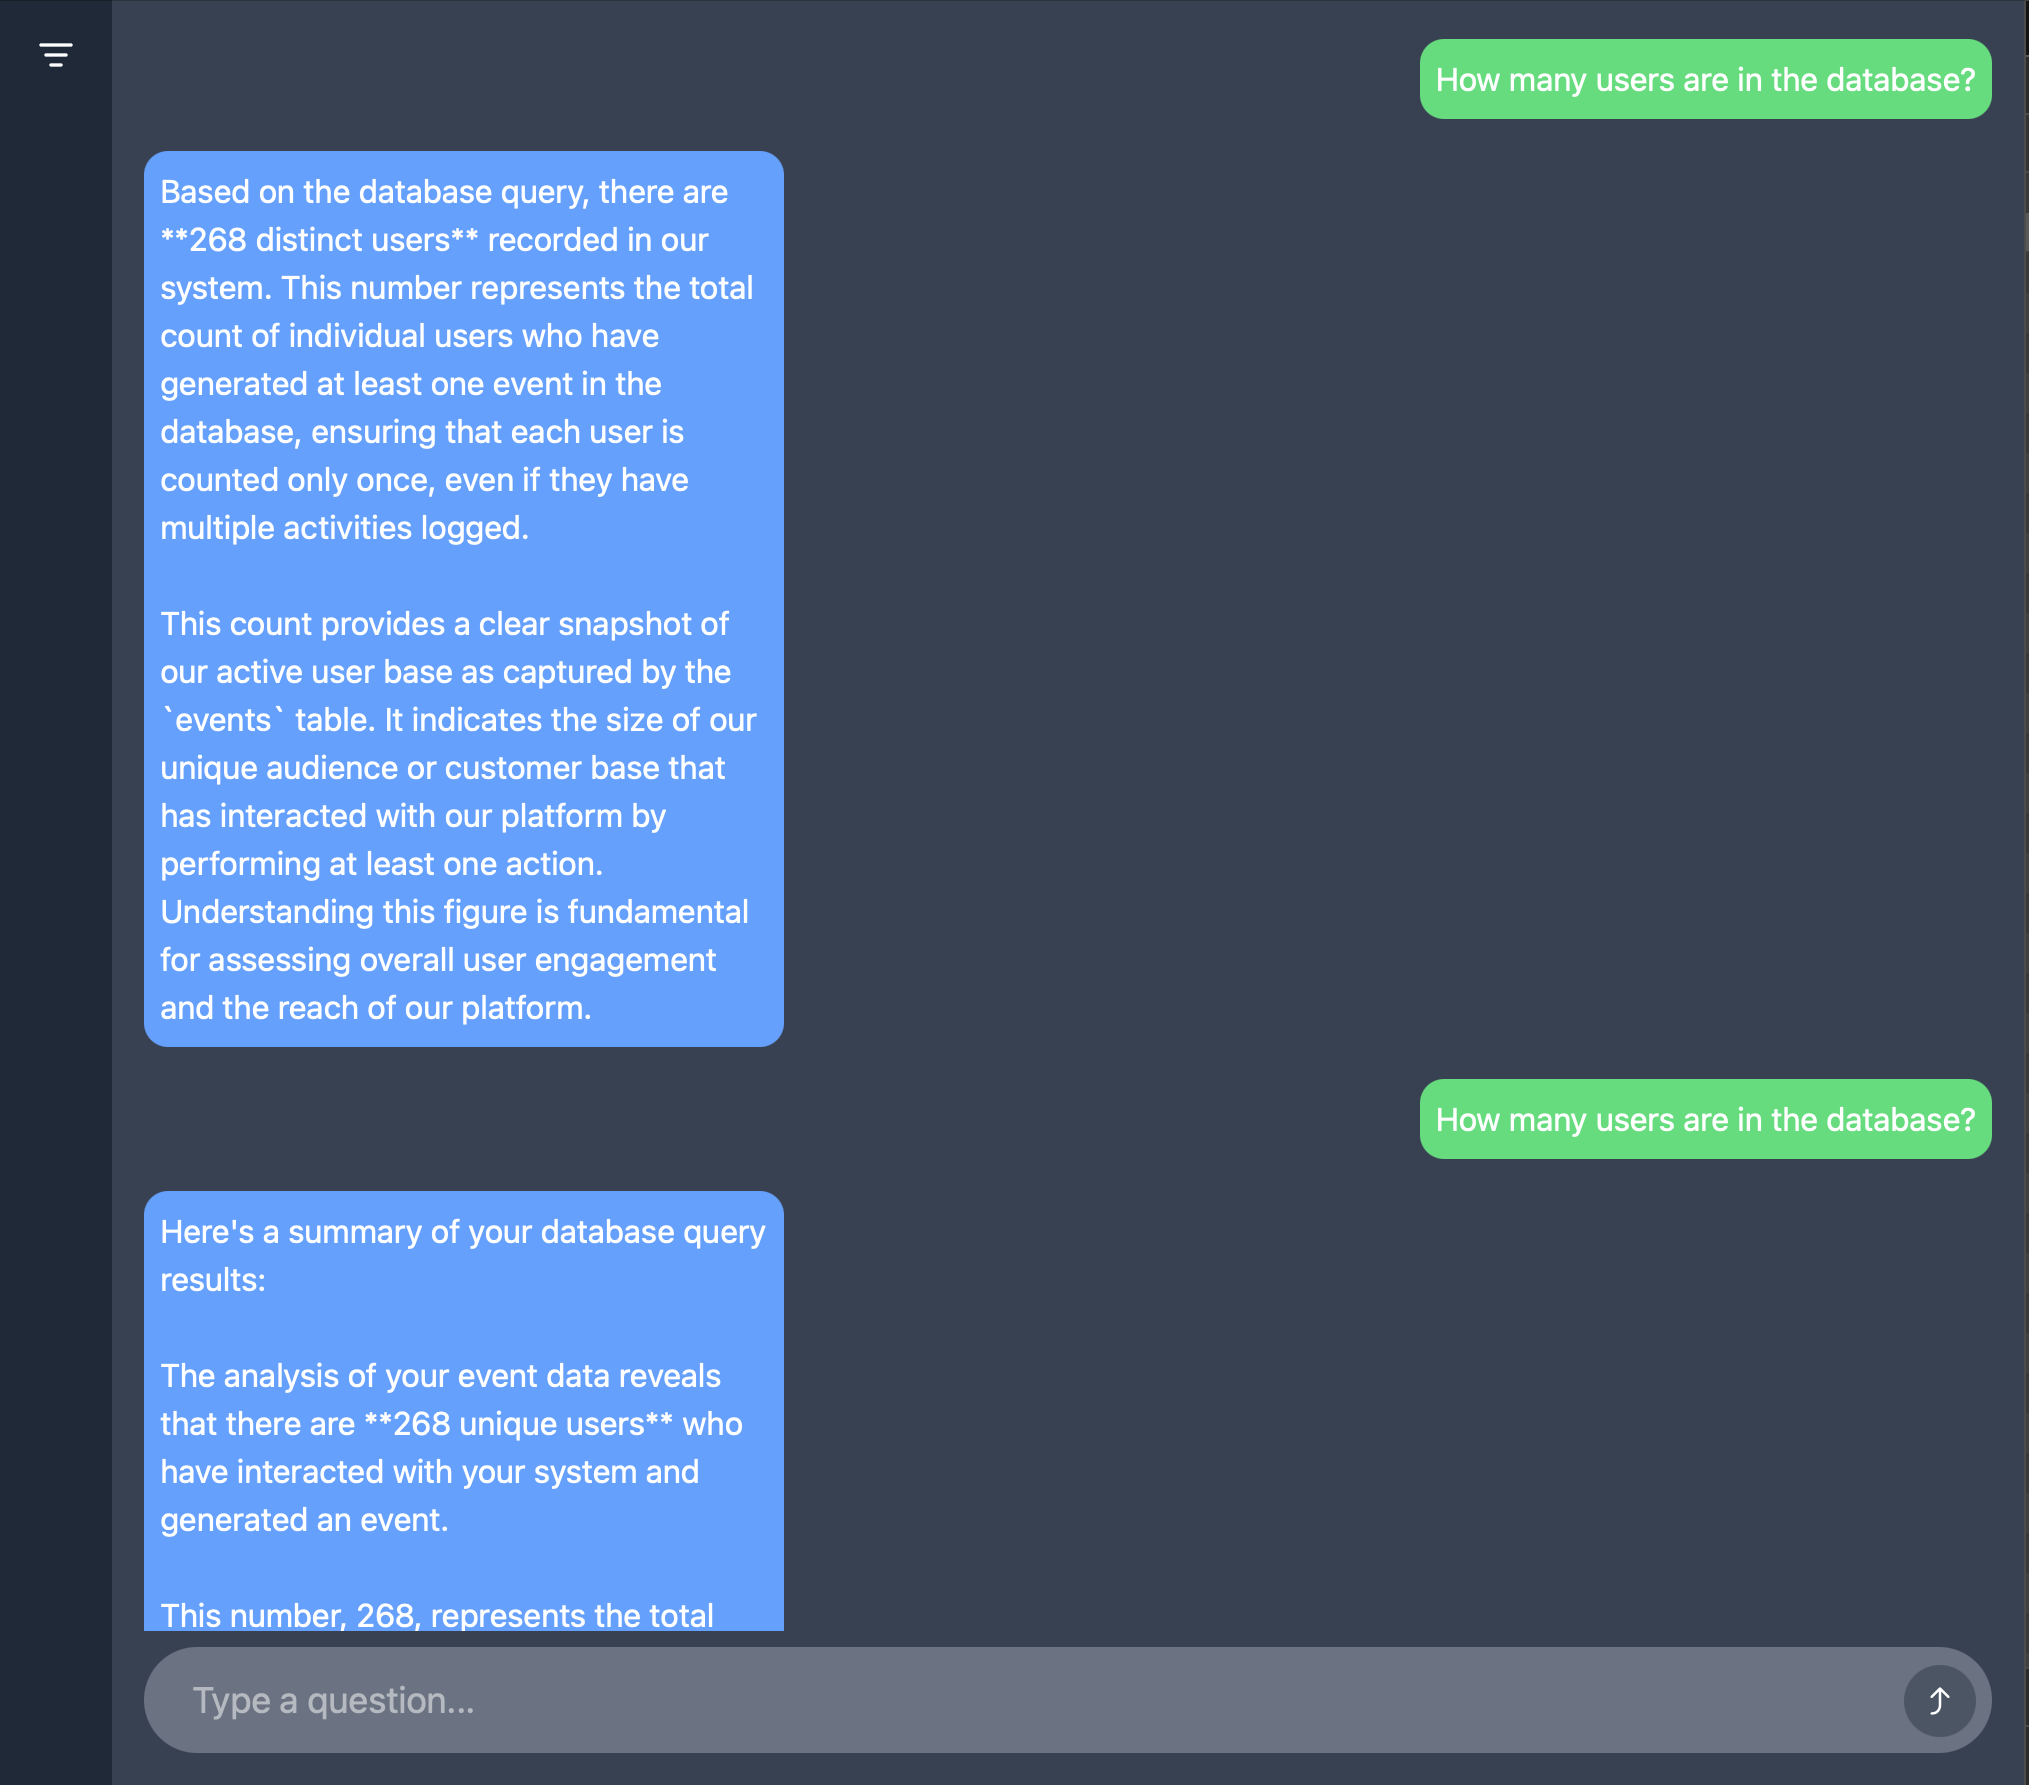
\includegraphics[width=0.8\textwidth]{chat_example.png}
\caption{Ukážka chatového rozhrania}
\end{figure}

\subsubsection{Správa pripojenia k databáze}

Používateľ môže databázu pripojiť alebo odpojiť pomocou tlačidla v bočnom paneli.  
Stav pripojenia sa vizuálne zobrazuje priamo na tlačidle:
\begin{itemize}
    \item \textbf{Connect Database} - databáza nie je pripojená,
    \item \textbf{Disconnect Database} - databáza je pripojená.
\end{itemize}


\begin{figure}[H]
\centering
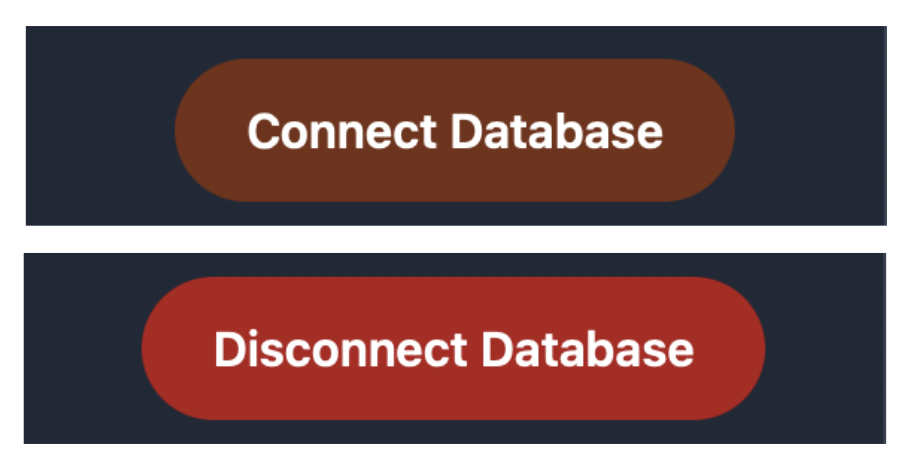
\includegraphics[width=0.45\textwidth]{database_button.png}
\caption{Stav pripojenia k databáze zobrazený na tlačidle}
\end{figure}

\subsubsection{Modálne okno}

Modálne okno slúži na zadanie údajov potrebných na pripojenie k databáze, ako sú hostiteľ, port, používateľské meno, heslo a názov databázy. Počas pripájania sa používateľovi zobrazuje stav \textbf{Connecting...}, aby vedel, že sa proces práve vykonáva. V prípade chyby sa zobrazí chybová hláška, ktorá informuje o neúspešnom pripojení.


\begin{figure}[H]
\centering
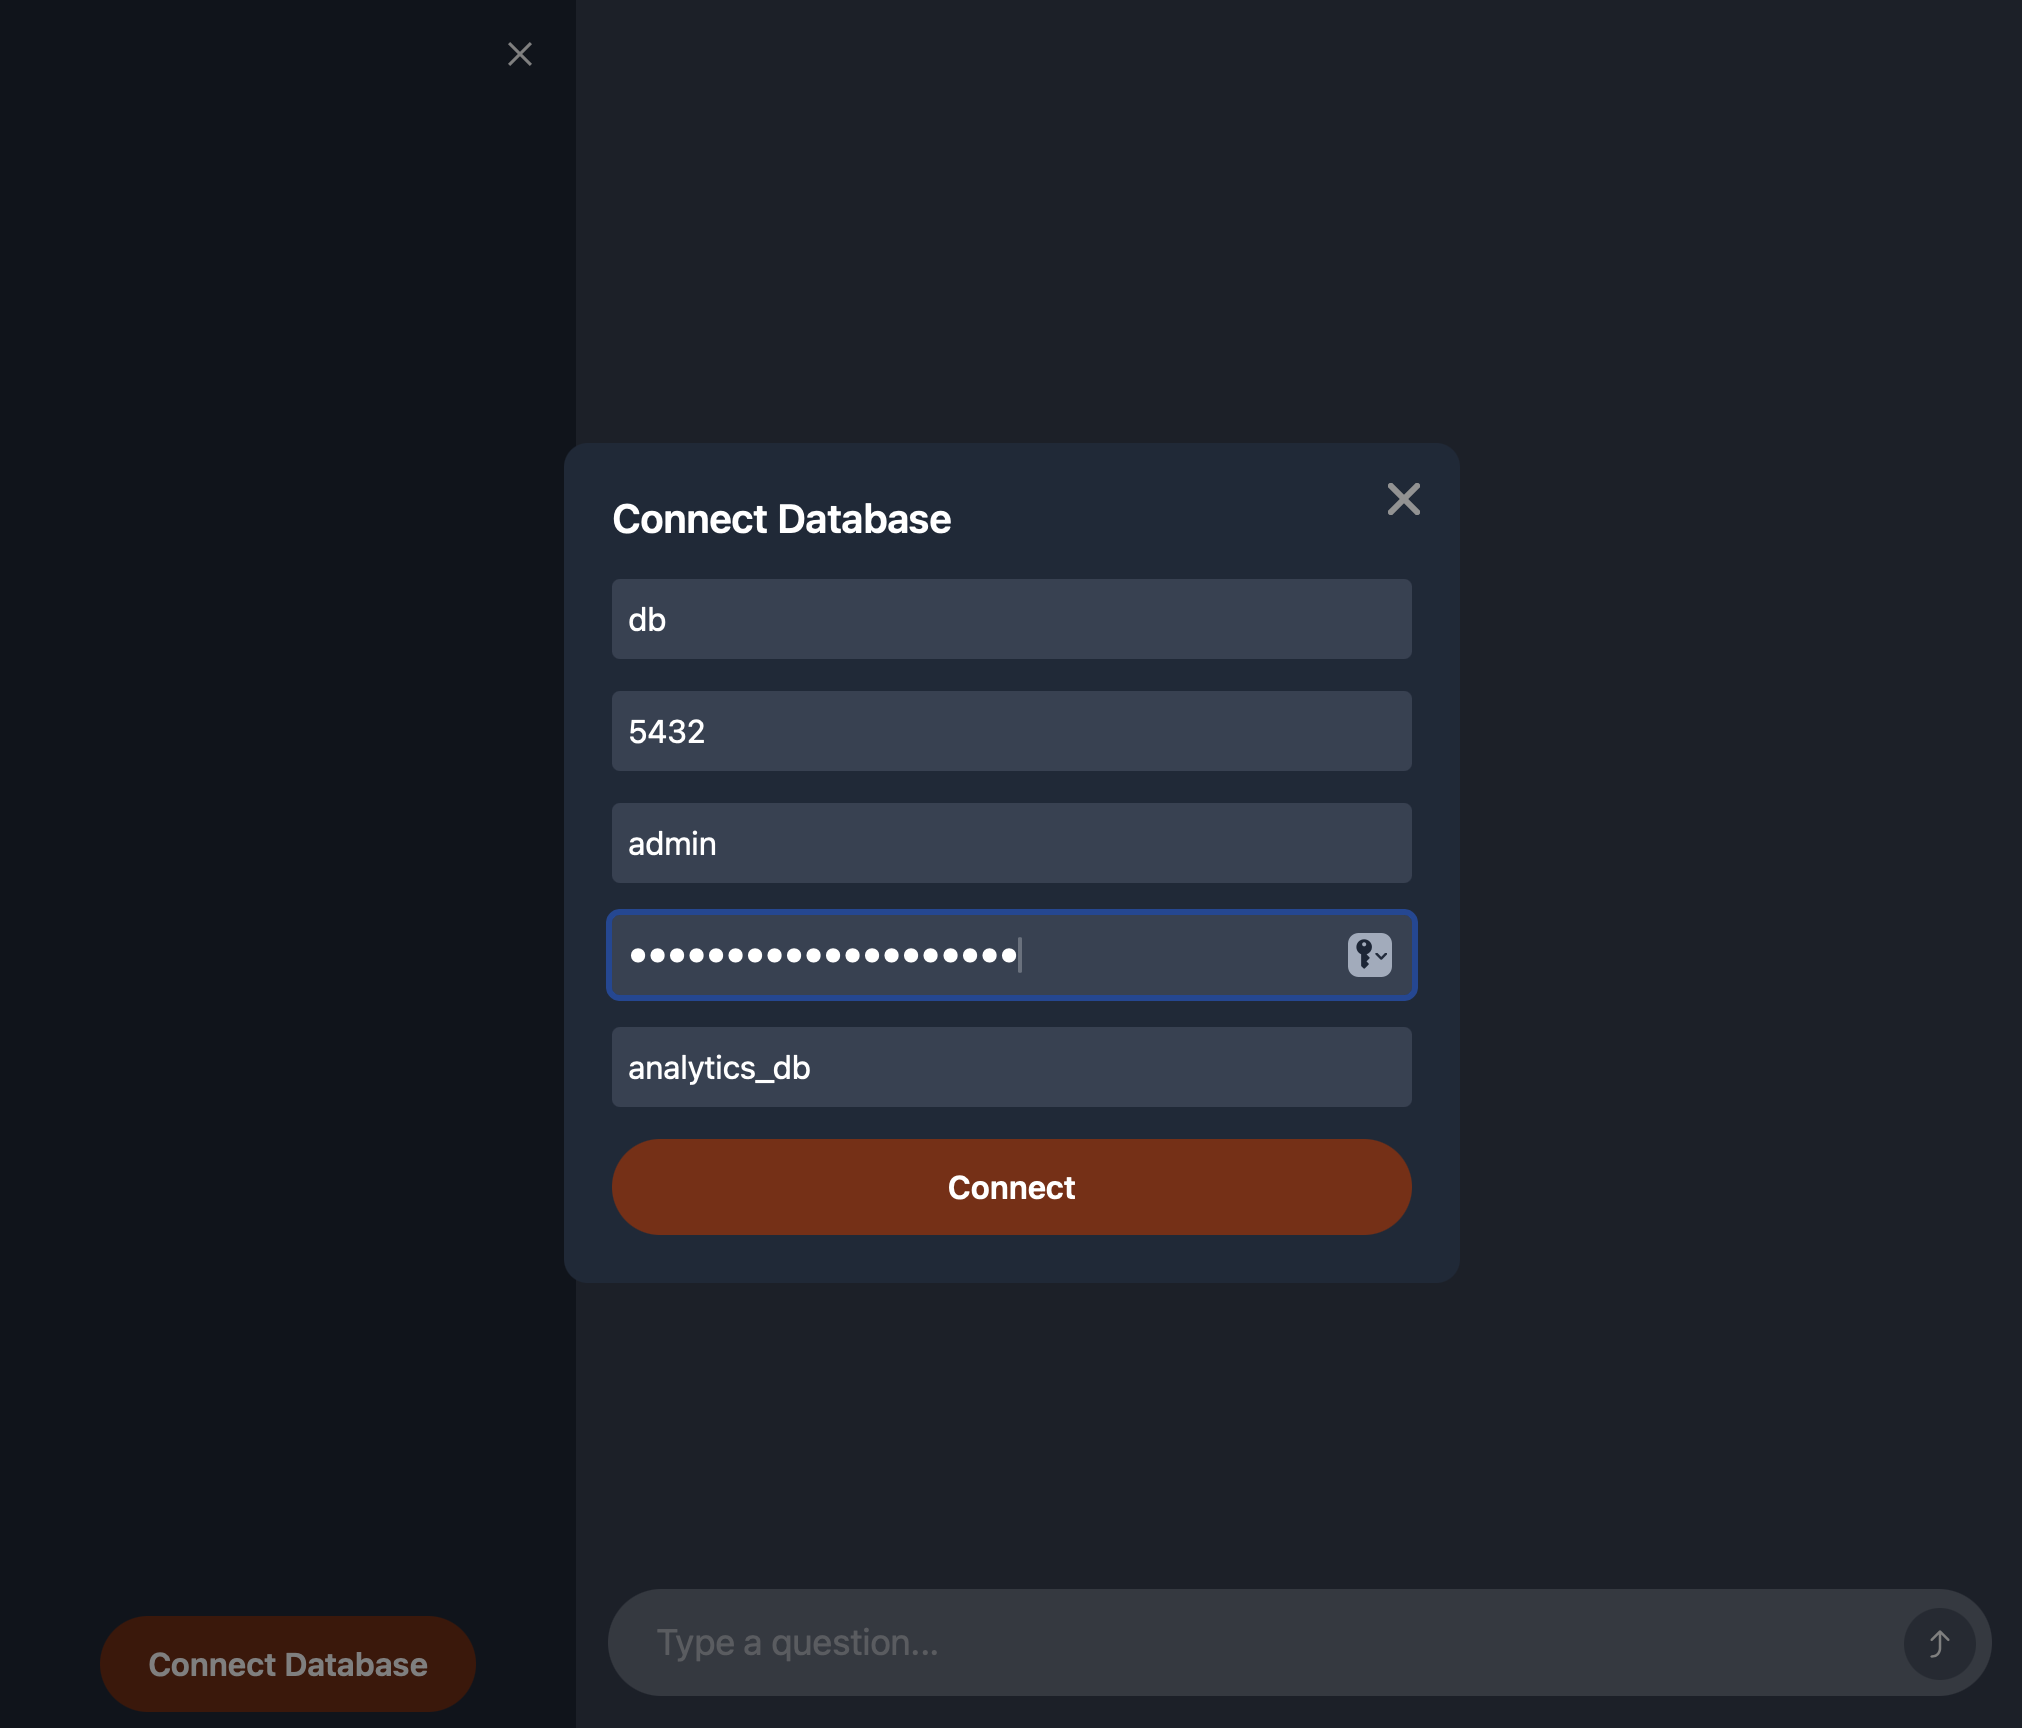
\includegraphics[width=0.9\textwidth]{database_modal.png}
\caption{Ukážka modálneho okna pre pripojenie databázy}
\end{figure}


\clearpage
\section*{Použitie nástrojov umelej inteligencie}

Pri vypracovaní projektu sme využili nasledujúce AI nástroje ako podporné prostriedky:

\begin{itemize}
    \item \textbf{Claude Opus 4.5 (Anthropic, 2025):} Využitý pri návrhu architektúry systému, code review a~optimalizácii kódu.
\end{itemize}
\begin{itemize}
    \item \textbf{Claude Sonnet 4.5 (Anthropic, 2025):} Využitý pri návrhu architektúry systému, code review a~optimalizácii kódu. Pomáhal s~formuláciou systémových promptov pre LLM komponenty.
\end{itemize}
\begin{itemize}
    \item \textbf{GPT-4.1 (OpenAI/Azure, 2025):} Integrovaný priamo v~systéme ako Query Generator pre transformáciu prirodzeného jazyka na SQL dotazy.
\end{itemize}

\begin{itemize}
    \item \textbf{Gemini 2.5 Flash (Google, 2025):} Integrovaný v~systéme ako Response Summarizer pre generovanie zrozumiteľných textových sumarizácií výsledkov dotazov.
\end{itemize}


\clearpage

\section*{Zdroje}

\begin{enumerate}
    \item FastAPI Documentation. (2025). \textit{FastAPI - Modern, Fast Web Framework}. \\
    \url{https://fastapi.tiangolo.com/}
    
    \item React Documentation. (2025). \textit{React - A JavaScript Library for Building User Interfaces}. \\
    \url{https://react.dev/}
    
    \item OpenAI. (2025). \textit{GPT-4 API Documentation}. \\
    \url{https://platform.openai.com/docs/}
    
    \item Google Cloud. (2025). \textit{Vertex AI - Gemini API}. \\
    \url{https://cloud.google.com/vertex-ai/docs/generative-ai/}
    
    \item PostgreSQL Global Development Group. (2025). \textit{PostgreSQL Documentation}. \\
    \url{https://www.postgresql.org/docs/}
    
    \item SQLAlchemy Documentation. (2025). \textit{SQLAlchemy - The Database Toolkit for Python}. \\
    \url{https://docs.sqlalchemy.org/}
    
    \item Docker Documentation. (2025). \textit{Docker Docs}. \\
    \url{https://docs.docker.com/}
    
    \item Redis Documentation. (2025). \textit{Redis Documentation}. \\
    \url{https://redis.io/documentation}

    \item Oracle Database Documentation. (2026). \textit{Oracle Database Documentation}.
    \url{https://docs.oracle.com/en/database/}

    \item Microsoft SQL server Documentation. (2026). \textit{SQL Server technical documentation}.
    \url{https://learn.microsoft.com/en-us/sql/sql-server/?view=sql-server-ver17}

    \item Medium (2023). \textit{Building Fast and Robust APIs with FastAPI and SQL Databases}. \\
    \url{https://medium.com/towards-data-engineering/fastapi-with-sql-1c7852ccbf21}
    
    \item Budibase. (2023). \textit{How to Integrate Multiple Databases}. \\
    \url{https://budibase.com/blog/data/how-to-integrate-multiple-databases/}
    
    \item Vite Documentation. (2025). \textit{Vite - Next Generation Frontend Tooling}. \\
    \url{https://vitejs.dev/}
    
    \item Tailwind CSS Documentation. (2025). \textit{Tailwind CSS - A Utility-First CSS Framework}. \\
    \url{https://tailwindcss.com/docs}
    
    \item Axios Documentation. (2025). \textit{Axios - Promise Based HTTP Client}. \\
    \url{https://axios-http.com/docs/intro}
    
    \item React Hooks Documentation. (2025). \textit{React Hooks - State and Lifecycle in Functional Components}. \\
    \url{https://react.dev/reference/react/hooks}
    
    \item Brown, T., et al. (2020). \textit{Language Models are Few-Shot Learners}. \\
    \url{https://arxiv.org/abs/2005.14165}
    
    \item Rajkumar, N., et al. (2022). \textit{Evaluating the Text-to-SQL Capabilities of Large Language Models}. \\
    \url{https://arxiv.org/abs/2204.00498}
    
    \item Pourreza, M., \& Rafiei, D. (2024). \textit{DIN-SQL: Decomposed In-Context Learning of Text-to-SQL}. \\
    \url{https://arxiv.org/abs/2304.11015}
\end{enumerate}

\end{document}